\section{Resoluci\'on del problema}

\subsection{Gram\'atica}

La gram\'atica resultante es: 

\begin{verbatim}
G = <Vn,Vt,Program,P>
\end{verbatim}

Donde:
\begin{verbatim}
Vt = { num, var, =, +, -, *, /, ^, &&, ||, !, ==, <, >, <= ,>=,(,),
{,},,,.,if,then,else,while,pi,function,plot,for,return} 

Vn = { Program, Funcs, Func, StatementsBlock, Statements, Statement, 
Args, BoolExp, Exp, CallArgs }

P = 
    Program : Funcs plot
            '(' var '(' CallArgs ')'  ',' var '(' CallArgs ')'  ')'
            for var '=' Exp '.' '.' Exp '.' '.' Exp
                

    Funcs : Func                 
          | Func Funcs           
    
    Func : function var '(' Args ')' StatementsBlock 
    
    StatementsBlock : Statement  
                    | '{' Statements '}'
    
    Statements : Statement       
               | Statement Statements 
    
    Statement : var '=' Exp      
              | if BoolExp then StatementsBlock else StatementsBlock 
              | if BoolExp then StatementsBlock 
              | while BoolExp StatementsBlock 
              | return Exp       
    
    Args :                       
         | var                   
         | var ',' Args          
    
    BoolExp : BoolExp '&&' BoolExp 
            | BoolExp '||' BoolExp 
            | '!' BoolExp        
            | Exp '==' Exp       
            | Exp '>' Exp        
            | Exp '<' Exp        
            | Exp '>=' Exp       
            | Exp '<=' Exp       
    
    Exp : Exp '+' Exp            
        | Exp '-' Exp            
        | Exp '*' Exp            
        | Exp '/' Exp            
        | Exp '^' Exp            
        | '(' Exp ')'            
        | '-' Exp
        | num                    
        | var                    
        | var '(' CallArgs ')'   
        | pi                     
    
    CallArgs :                   
             | Exp               
             | Exp ',' CallArgs  
\end{verbatim}



Es sencillo ver que esta gram\'atica es ambigua y no define precedencias. 
Estos problemas son solucionados en \textsc{Happy} mediante precedencias.

La gram\'atica est\'a definida en el archivo \texttt{Grammar.y}

\subsection{Lexer}

En el \textit{lexer} definimos los tokens utilizando las siguientes reglas:
\texttt{<state> Vt \{ action \}}. \texttt{state} es el estado en el cual debe estar
el \textit{lexer} para poder parsear el \texttt{Vt}. Los estados permiten modelar distintas
reglas para un mismo \texttt{Vt}, dependiendo que otros s\'imbolos se hayan encontrado
antes. \texttt{action} es la acci\'on a tomar cuando se encuentra el s\'imbolo.

Nuestra implemtaci\'on utiliza dos tipos de acciones: \texttt{begin} que permite
cambiar el estado actual, y \texttt{lex} que crea un Token. A continuaci\'on damos
dos ejemplos de esto:

Las siguientes reglas indican que se deben ignorar los comentarios multil\'inea

\begin{verbatim}
<0>       "/*"                     { begin comment }
<comment> [^ \* ]*                 ;
<comment> "*/"                     { begin 0 }
\end{verbatim}

Un ejemplo de $lex$ es generar el token que indica se est\'a realizando una
suma:

\begin{verbatim}
<0>  \+                            { lex' TokenPlus }
\end{verbatim}

Todos los tokens est\'an definidos en el archivo \texttt{Tokens.x}


\subsection{Parser}

Las asociaciones de los operadores y sus precedencias se resuelven 
indicando a \textsc{Happy} como son las mismas mediante reglas de la forma
\texttt{\% left|right|nonassoc  Vt}, donde \texttt{left} indica que el terminal asocia a izquierda,
\texttt{right} que asocia a derecha y \texttt{nonassoc} que no son asociativos. El orden en que
ponemos estas reglas indica la precedencia (de menor precedencia, a mayor precedencia).

Como bien indicamos, algunas de las producciones de la gram\'atica hacen
que sea ambigua, por ejemeplo, el \textit{if then else}. Se espera que los $else$
se asocien a los $if$ m\'as cercanos, para esto utilizamos la regla:
\begin{verbatim}
%right then else  
\end{verbatim}


En el caso de los operadores l\'ogicos, eliminamos la ambig\"uedad 
asociando a izquierda y dando mayor precedencia a la negaci\'on, luego
a la conjunci\'on y, por \'ultimo, a la disyunci\'on.
\begin{verbatim}
%left '||'     
%left '&&'   
%left '!'    
\end{verbatim}

Estas reglas se encuentran al inicio del trchivo \texttt{Grammar.y} 

Lo siguiente que necesita el generador de \textit{parser} es que escribamos la gram\'atica 
como una gram\'atica de atributos, haciendo que, por cada producci\'on,
se vaya generando una estructura. Estructura que luego ser\'a analizada
por el int\'erprete para dar ejecutar el programa.

La estructura se encuentra definida en el archivo \texttt{Language.hs} y
es la siguiente:

\begin{verbatim} 
type Arg = String
type Var = String
type Name = String

data Program = Program [Func] Exp Exp Var Exp Exp Exp

data Func = Func Name [Arg] [Statement]

data Statement = StmtReturn Exp
               | StmtAssign Var Exp
               | StmtIf BoolExp [Statement] [Statement]
               | StmtWhile BoolExp [Statement]

data Exp = Plus Exp Exp
         | Minus Exp Exp
         | Times Exp Exp
         | Div Exp Exp
         | Pow Exp Exp
         | Negate Exp
         | Brack Exp
         | Num Double
         | Var String
         | Call Name [Exp]
         | Pi

data BoolExp = And BoolExp BoolExp
             | Or  BoolExp BoolExp
             | Not BoolExp
             | Eq  Exp Exp
             | Gtr Exp Exp
             | Lwr Exp Exp
             | Geq Exp Exp
             | Leq Exp Exp
\end{verbatim}

Un ejemplo de c\'omo se usa en la gram\'atica de atributos es:

\begin{verbatim}
Exp : Exp '+' Exp            { Plus $1 $3 }
    | num                    { Num $1 }
\end{verbatim}

Al usar la producci\'on \texttt{Exp ${\rightarrow}$ num}, creamos un 
\texttt{Num num}, y al usar \texttt{Exp ${\rightarrow}$ Exp+Exp} creamos
\texttt{Plus Exp1 Exp2}, donde \texttt{Exp1} y \texttt{Exp2} son las expresiones creadas
al ser parseado cada una de las \texttt{Exp}.

En este punto es interesante destacar que el paradigma funcional de \textsc{Haskell}
empieza a jugar un rol muy importante. Esto puede verse, por ejemplo, en la producci\'on:
\begin{verbatim}
CallArgs :                   { [] }
         | Exp               { $1:[] }
         | Exp ',' CallArgs  { $1:$3 }
\end{verbatim}

Vemos como se genera la lista de argumentos de forma totalmente natural, pues la recursi\'on
estructural es el punto fuerte de este tipo de lenguajes.


\subsection{Int\'erprete y peque\~no manual del programa}

\subsubsection{Funcionamiento del programa}

El int\'erprete recibe un tira de caracteres como par\'ametro.
En general se escriben las funciones en un archivo y se pasa el contenido del
archivo al int\'erprete mediante \textit{stdin}.

Internamente el programa consta de un \textit{lexer}, un \textit{parser} y el
int\'erprete propiamente dicho.

El funcionamiento del \textit{parser} y el del \textit{lexer} ya fue detallado
anteriormente. Estos hacen uso de los tipos abstractos de datos:
\begin{itemize}
    \item \texttt{Program}
    \item \texttt{Func}
    \item \texttt{Statement}
    \item \texttt{Exp}
    \item \texttt{BoolExp}
\end{itemize}

Una vez ejecutado el \textit{parser} el int\'erprete recibe un \texttt{Program}.
El int\'erprete, entonces, llama a la funcion \texttt{evalProg} con ese 
\texttt{Program} como argumento.

Esta funci\'on chequea que no haya una funci\'on declarada m\'as de una vez
y, si no hubiese errores, evalua la funcion explicitada en la secci\'on
\texttt{plot} del c\'odigo pasado por \textit{stdin} en cada uno de los puntos
del rango explicitado.

Para esto se utiliza la funci\'on \texttt{evalFunc}. A una funci\'on se la
interpreta, b\'asicamente, como una lista de \texttt{Statement}s.
Luego, para evaluarla, se necesita evaluar cada \texttt{Statement}
manteniendo cierto estado de las variables que aparecen en la funci\'on.

Para esto se tiene al tipo \texttt{PartialEval} que puede ser uno de dos
tipos: un \texttt{EnvFunc} o un n\'umero (resultado).
La idea es que cada \texttt{Statement} toma un \texttt{PartialEval} y
devuelve un \texttt{PartialEval}. Si justo se tratara de un \texttt{Statement}
de tipo \textit{return}, el resultado ser\'a un n\'umero. Pero si se tratara
de una asignaci\'on a una varible, simplemente devolvera un contexto (
\texttt{EnvFunc}) con el contexto anterior, modificando (o agregando) el valor
de la variable en cuesti\'on.

Llegado el final de la funci\'on (consumida toda la lista de \texttt{Statement}s)
el int\'erprete da un error, pues toda funci\'on debe retornar un valor
(llegar a un \textit{return}).

Es intersante notar que chequear si la funci\'on llega a un \textit{return} o
no, no puede realizarse est\'aticamente. M\'as a\'un, se trata del
\textit{halting problem}, con lo cual un programa podr\'ia no tener \textit{return}
declarados y colgarse. Podr\'ia tambi\'en tenerlos y colgarse, y podr\'ia
tenerlos o no tenerlos y a\'un as\'i quedarse sin instrucciones para ejecutar
(en el caso de tener un \textit{if} o \textit{while}). Con lo cual no tiene
sentido hacer ninguno de estos chequeos, y son problemas que solo pueden
detectarse en \textit{runtime}.

Para poder evaluar \texttt{Statement}s del tipo asignaciones usualmente deben
evaluarse expresiones. Para esto est\'a la funci\'on \texttt{evalExp}.
Esta funci\'on es una recursi\'on (o \textit{fold}) totalmente estandar.
De forma an\'aloga tenemos la funci\'on \texttt{evalBoolExp}, que sirve
para la guarda del \textit{if} y la del \textit{while}.

\subsubsection{Diagrama de clases}
Es complicado realizar un diagrama de clases de una implementaci\'on en un lenguaje
que, justamente, no implementa clases. De todas maneras realizamos un diagrama
teniendo en mente una posible traducci\'on de nuestra implementaci\'on a un dise\~no
basado en clases.

Para comprenderlo en profundidad es recomendable tener a mano el c\'odigo y sobre
todas las cosas las declaraciones de los tipos abstractos de datos y las signaturas
de las funciones implementadas. En \textsc{Haskell} las signaturas suelen dar casi
toda la informaci\'on relevante de una funci\'on.

\begin{figure}[!ht]
    \centering
    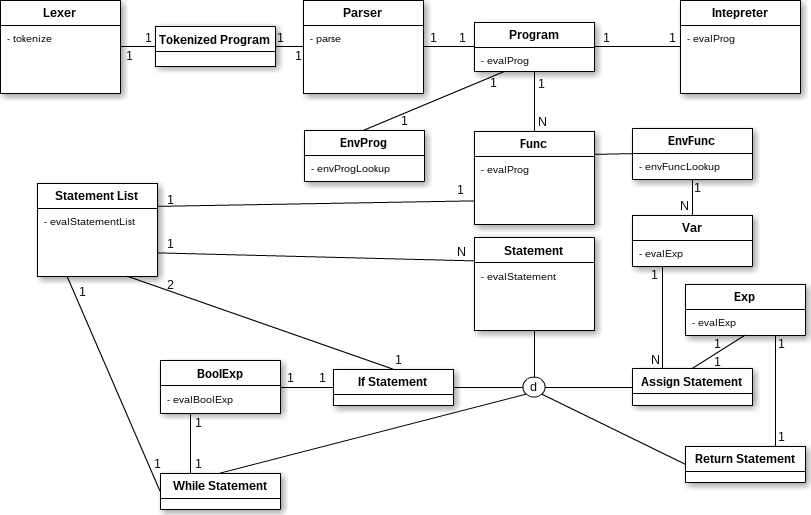
\includegraphics[width=\textwidth]{ClassDiagram.png}
    \caption{Diagrama de clases de la implementaci\'on}
\end{figure}

\begin{figure}[!ht]
    \centering
    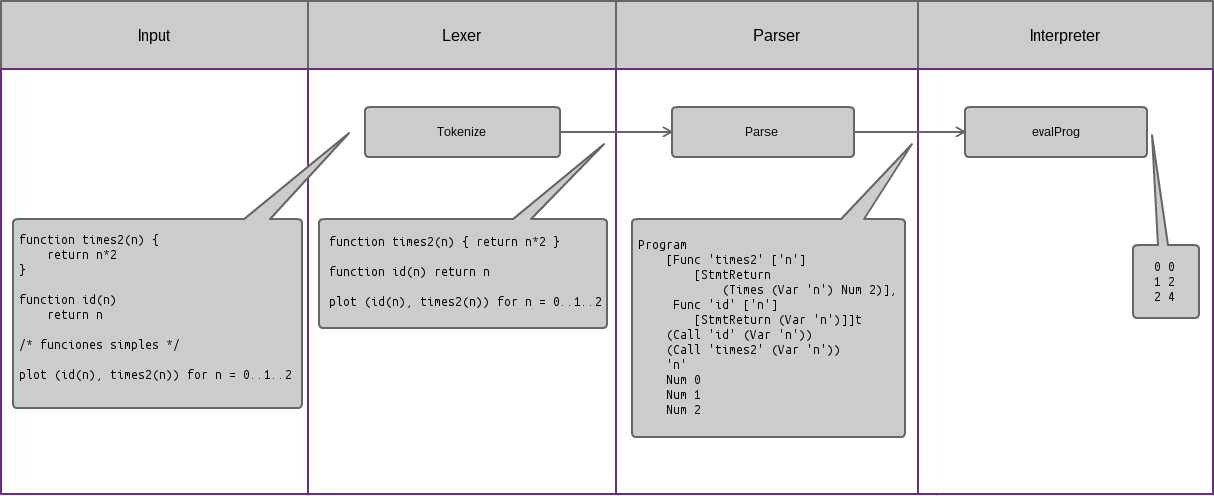
\includegraphics[width=\textwidth]{Flowchart.png}
    \caption{Ejemplo de ejecuci\'on}
\end{figure}


\subsubsection{Modo de uso}
Para compilar el int\'erprete es necesario contar con las aplicaciones 
\textit{Alex}, \textit{Happy} y \textit{ghc} instaladas\footnote{Para esto
puede resultar c\'omodo el programa \textsc{Cabal} que facilita el manejo
de paquetes relacionados con \textsc{Haskell}.}. En la carpeta
\textit{src} incluimos un \textit{Makefile} que genera el ejecutable
\textit{Interprete}.

Para utilizarlo basta con pasarle por \textit{stdin} el c\'odigo a ejecutar.
\begin{verbatim}
cat codigo.cod | ./Interprete
\end{verbatim}
A esto podemos agregarle mediante un \textit{pipe} las instrucci\'on para
\textsc{gnuplot} brindada por la c\'atedra.
